\chapter{Impact of the scale setting in hadronic computations}
\label{ch_charm}

%%%%%%%%%%%%%%%%%%%%%%%%%%%%%%%%%%%%%%%%%%%%%%%%%%%%%%%%%%%
%%%%%%%%%%%%%%%%%%%%%%%%%%%%%%%%%%%%%%%%%%%%%%%%%%%%%%%%%%%
%%%%%%%%%%%%%%%%%%%%%%%%%%%%%%%%%%%%%%%%%%%%%%%%%%%%%%%%%%%
%%%%%%%%%%%%%%%%%%%%%%%%%%%%%%%%%%%%%%%%%%%%%%%%%%%%%%%%%%%

\section{Introduction}
\label{ch_qm:sec:introduction}

In this Chapter we discuss hadronic computations involving the charm quark following our work~\citep{charm}, with special emphasis on the impact on these results of the scale $t_0$ we obtained in Chapter \ref{ch_ss}. In particular, we will see that with the high precision result we obtained in eq.~(\ref{ch_ss:eq:t0ph_c}) we can quote results for the renormalized charm quark mass and $D_{(s)}$ charmed mesons decay constants where the scale $t_0$ is not the dominant source of uncertainty. 

For the extraction of charm observables we rely entirely on the mixed action setup, exploiting automatic $\mathcal{O}(a)$ improvement for valence observables, ensured by our mixed action setup once the matching of the sea and valence sectors, in addition to the tune to maximal twist explained in Sec.~\ref{ch_ma:sec:matching} are performed. This helps in keeping under control large discretization effects associated to the heavy mass of the charm quark. 

In Sec. \ref{sec:matching_charm} we discuss the details of our strategy to match the charm quark mass to its physical value. In Sec.~\ref{sec:mc} we discuss chiral-continuum extrapolations of the renormalized charm quark mass and present our results for this quantity at the physical point after performing a model average of the different possible extrapolations. In Sec.~\ref{sec:fDs} we present our results for the charmed mesons $D_{(s)}$ decay constants, showing the contribution to the final uncertainty coming from the determination of the scale $t_0$. For a complete discussion of these results we refer to our work~\citep{charm}. 

In addition to these charmed mesons computations, in Appendix~\ref{apex_light_qm} we show some preliminary analysis of the light and strange quark masses. 


\section{Matching of the charm quark mass}
\label{sec:matching_charm}

In Sec.~\ref{ch_ma} we performed the matching of the sea and valence sectors of our mixed action for the light and strange flavors, in addition to tuning to maximal twist. Once the valence parameters were determined to ensure these conditions, an independent set of computations of heavy propagators was performed for the study of charm physics. Heavy propagators are computed at three different values of the twisted  mass $\mu_c^{(i)}$ around the physical charm region for the main set of ensembles, while for a subset of them only two masses have been used, so that observables are interpolated at the physical value of the charm quark mass. In order to fix the charm quark mass to its physical value, we use different combinations of mesons masses $m_H$ matched to their physical values. Since the charm is partially quenched, this matching procedure involves observables with only valence charm quark propagators. 
%

We study two different charm scale settings based on two choices of $m_H^{(i)},~i=1,2$, and will often be expressed in units of $\sqrt{8t_0}$ as $\phi_H^{(i)} = \sqrt{8t_0}m_H^{(i)}$.
%

The first possibility we explore, corresponding to $\phi_H^{(1)}$, consists in using the flavor average meson mass combination
\begin{equation}
        m_H^{(1)} = m_{\overline{H}} \equiv \frac{2}{3} m_H + \frac{1}{3}m_{H_s},
        \label{eq:fl_av_matching}
\end{equation}
built from heavy-light $H$ and heavy-strange $H_s$ pseudoscalar meson masses with heavy-quark masses in the neighborhood of the charm.
%
Since we mass shifted\footnote{In the case of charmed observables like the ones in this Chapter, the mass shift was performed in a similar manner to what is discussed in Sec. \ref{ch_ma:sec:chiral_traj}, but this time using the dedicated measurements of the mass derivatives for each ensemble, instead of parametrizing them as functions of $\phi_2$ and the lattice spacing.} the considered CLS ensembles in order to impose a constant value of $\phi_4$ (see eq.~(\ref{ch_ma:eq:phi4})), we expect the flavor average combination $\phi_H^{(1)}$ to remain fairly constant along the chiral trajectory. The physical value of $m_H^{(1), \mathrm{ph}}$ is obtained by setting $m_{H_{(s)}}$ to the following prescription for the isoQCD values of $D_{(s)}$ meson masses,
%
\begin{equation}
    m_D^{\mathrm{isoQCD}} = 1867.1(2.6)  \ \mathrm{MeV}, \qquad m_{D_s}^{\mathrm{isoQCD}} = 1967.1(1.3) \ \mathrm{MeV}.
\label{eq:DsisoQCDinputs}
\end{equation}
%
The uncertainties in these isoQCD values are chosen to cover the deviation with respect to the experimental values~\cite{ParticleDataGroup:2022pth} of the $D^{\pm}$ and $D_s^{\pm}$ meson masses, $m_{D^\pm}^{\mathrm{exp}} = 1869.66(5) \ \mathrm{MeV}$ and $m_{D_s^\pm}^{\mathrm{exp}} = 1968.35(7) \ \mathrm{MeV}$, respectively. We observe that the larger uncertainty in the isoQCD inputs of the $D$ and $D_s$ meson masses in eq.~(\ref{eq:DsisoQCDinputs}) --- as compared to the corresponding experimental values --- does not induce a significant increase in the uncertainties of our target results. The input values in eq.~(\ref{eq:DsisoQCDinputs}) lead to the following flavor averaged meson mass,
%
\begin{equation}
         m_H^{(1), \mathrm{ph}} = m_{\overline{D}} = 1900.4(1.8) \ \mathrm{MeV}\,.
\end{equation}
% 

The second strategy, corresponding to $\phi_H^{(2)}$, is to consider the mass-degenerate pseudoscalar meson mass $m_{\eta_h}^{\mathrm{conn}}$ extracted from the quark-connected two-point correlation function made of heavy quark propagators with a mass in the neighbourhood of the charm mass,
%
\begin{equation}
  m_H^{(2)} = m_{\eta_h}^{\mathrm{conn}}\,.
\label{eq:etac_matching}
\end{equation}
%
The physical value for this mass, $m_H^{(2), \mathrm{ph}}$,  is set from the experimental value of the $\eta_c$ meson mass~\cite{ParticleDataGroup:2022pth}, $m_{\eta_c}^{\mathrm{exp}} = 2983.9(4)\,$ MeV, from which a correction of about 6 MeV, with 100\% error, is subtracted to account for the absence of quark-disconnected diagrams and QED effects~\cite{deForcrand:2004ia, Donald:2012ga,Colquhoun:2015oha,Hatton:2020qhk,Colquhoun:2023zbc}. Specifically, we employ, 
%
\begin{equation}
  m_H^{(2), \mathrm{ph}} = m_{\eta_c}^{\mathrm{conn}} = 2978(6) \ \mathrm{MeV}\,.
\end{equation}
%
One potential advantage of this choice of matching observable is that the overall precision of the $\eta_c^{\mathrm{conn}}$ meson mass is substantially better than the one for heavy-light meson masses, as it does not suffer from the increase in noise-to-signal ratio with Euclidean time.
%

%
Any of these matching conditions can in principle be imposed ensemble by ensemble, even away from the physical point.
%
However, by doing so we would as a result build in the charm quark mass a dependence on the value of the reference scale $t_0^{\mathrm{ph}}$, as well as $\mathcal{O}(a^2)$ effects coming from the specific choice of $m_H$.
%
To avoid this, we have opted instead for setting the physical charm quark mass jointly with the chiral-continuum extrapolation, in a similar way as the one we employ to hit the physical point in the light and strange sector.
%
What this means in practice is that the charm quark mass dependence of any given observable $\cO$ is parameterized as $\mathcal{O}(a, \phi_2, \phi_H^{(i)})$, and we perform a global fit to obtain its physical value $\mathcal{O}(0, \phi_2^{\mathrm{ph}}, \phi_H^{(i),\mathrm{ph}})$.
%
This will be the procedure applied below in the determination of the physical value of the charm quark mass and of the decay constants $f_D$ and $f_{D_s}$.
%

%%%%%%%%%%%%%%%%%%%%%%%%%%%%%%%%%%%%%%%%%%%%%%%%%%%%%%%%%%%
%%%%%%%%%%%%%%%%%%%%%%%%%%%%%%%%%%%%%%%%%%%%%%%%%%%%%%%%%%%
%%%%%%%%%%%%%%%%%%%%%%%%%%%%%%%%%%%%%%%%%%%%%%%%%%%%%%%%%%%
%%%%%%%%%%%%%%%%%%%%%%%%%%%%%%%%%%%%%%%%%%%%%%%%%%%%%%%%%%%

\section{Determination of the charm quark mass}
\label{sec:mc}

\subsection{Renormalized charm quark masses}

%
As discussed in Sec.~\ref{ch_foundation:subsec:tm}, in the Wilson tm regularization, renormalized quark masses can be easily retrieved from bare Lagrangian twisted masses. In our mixed-action setup the resulting $\mathcal{O}(a)$ improved expression for the renormalized  charm mass $\mu^{\textrm{R}}_c$ reads
\begin{equation}
	\mu^{\textrm{R}}_c=Z_P^{-1}(g_0^2,a\mu_{\textrm{ren}})\left[1+a\overline{b}_\mu\textrm{tr}\left(M_q^{(s)}\right)\right]\mu_c\,,
	\label{eq:renormalized_charm_mass}
\end{equation}
where $Z_P$ is the renormalization constant for the non-singlet
pseudoscalar density at some renormalization scale $\mu_{\textrm{ren}}$ as discussed in Sec.~\ref{ch_foundation:subsec:tm}.
%
The improvement coefficient $\overline{b}_{\mu}$ is suppressed by the trace of the sea quark mass matrix $\textrm{tr}\left(M_q^{(s)}\right)$ where only light quarks enter, and therefore it can be neglected because its natural value is well below the precision of the computation. Thus $\mathcal{O}(a)$ improved renormalized quark masses can be obtained by just applying the renormalization constants to the twisted masses $\mu_i$ in the Lagrangian.
%

The values of $Z_P$ are listed in Table~\ref{ch_observables:tab:Z} and were computed at a fixed renormalization scale $\mu_{\textrm{had}}=233(8)$ MeV. They allow to obtain renormalized quark masses for each of our ensembles, that can then
be used to determine the value of the charm quark mass in the continuum and at physical kinematics.
%
Contact with other renormalization schemes can then be made by computing the renormalization
group invariant (RGI) quark mass $M_c^{\mathrm{RGI}}$, using the continuum (flavor-independent)
ratio also computed in~\cite{Campos:2018ahf}
\begin{equation}
	\frac{M}{\overline{m}(\mu_{\mathrm{had}})} = 0.9148(88)\,.
	\label{eq:rgi_running_factor}
\end{equation}
%
Values of renormalized masses in another renormalization scheme can then be obtained by
using the perturbative value of $\frac{\overline{m}(\mu)}{M}$ at any convenient scale $\mu$.
%

%%%%

\subsection{Charm quark mass chiral-continuum fits}
\label{subsec:mc_chiral_continuum}

Having determined the  renormalized charm quark masses in the Schr\"odinger Functional scheme at the hadronic renormalization scale $\mu_{\mathrm{had}}$, $\mu_c^{\textrm{R}}$, for all the ensembles listed in Table \ref{apex_ensembles:tab:ens}, we can perform the chiral-continuum fits to obtain results in the continuum limit and at the physical point. The matching procedure of the light
and strange sectors is already devised so that the physical value of the kaon mass is recovered
at $\phi_2 = \phi_2^{\mathrm{ph}}$, where the physical value of $\phi_2$ is computed
with the isoQCD values of the pion mass quoted 
in~\cite{FlavourLatticeAveragingGroupFLAG:2021npn} (see eqs.~(\ref{ch_ss:eq:isoQCD})), and the physical scale $t_0^{\mathrm{ph}}$
is the one determined in eq.~(\ref{ch_ss:eq:t0ph_c}). The charm scale is matched through the two different
prescriptions described in Sec.~\ref{sec:matching_charm}. All quantities entering the fit
are made dimensionless through the appropriate power of the factor $\sqrt{8t_0}$,
and physical units for the final result are restored by using our value for $t_0^{\mathrm{ph}}$.

We parameterize the continuum dependence of the renormalized charm quark mass on $\phi_2$
and any of the $\phi_H^{(i)}$ with the functional form
\begin{equation}
	\sqrt{8t_0}\, \mu_c^{\textrm{R}}(a=0, \phi_2, \phi_H) = p_0 + p_1\phi_2 + p_2\phi_H\,.
	\label{eq:mc_continuum_parameterization}
\end{equation}
Based on the heavy quark effective theory expansion~\cite{Georgi:1990um} at lowest order,
we expect a linear dependence of the charmed meson masses as a function of the charm quark 
mass, hence the latter term in the ansatz. This assumption is supported by our data that show indeed a 
linear behavior in the charmed meson masses, as illustrated in Figure \ref{fig:mc_mh_dependence}. Note that this form is used only to describe the dependence
within a short interval in mass values, and interpolate the charm scale from points close by. When considering the pion dependence of the charm quark mass, we assume that the  leading order contributions exhibit a linear behavior in $\phi_2$. With the set of ensembles employed in this work we do not observe any deviations from the leading order term in the pion mass dependence.

Regarding the lattice spacing dependence of the charm quark mass, we assume the leading cutoff effects to 
be $\mathcal{O}(a^2)$, as discussed above. Corrections of odd order in $a$ are generically expected to be highly
suppressed at maximal twist, by way of the extension of the argument for automatic $\mathcal{O}(a)$
improvement; we thus include $a^4$ terms to account for deviations from linear behavior
in $a^2$. Finally, we allow for terms proportional to $m_\pi^2$ and to various powers of the charm
mass. The generic ansatz to parameterize lattice spacing dependence thus take the following form
\begin{equation}
	c_{\mu_c}(a, \phi_2, \phi_H) = \frac{a^2}{8t_0} \big(
	c_1 + c_2\phi_2 + c_3 \phi_H^2
	\big)
	+
	\frac{a^4}{(8t_0)^2}\big(
	c_4 + c_5\phi_H^2 + c_6 \phi_H^4
	\big).
	\label{eq:lattice_spacing_dependence}
\end{equation} 

In order to estimate the systematic effects arising from the model variation, we consider all the possible 
combinations where some of the $c_i$ coefficients vanish, save for $c_1$ which is always kept.
Furthermore, following~\cite{Heitger:2021apz}, we allow for cutoff effects to enter either linearly or 
non-linearly, viz.,
  \begin{align} 	\label{eq:tot_model}
 	\sqrt{8t_0}\mu_c^{R,\text{linear}}(a, \phi_2,\phi_H) &=
 	\sqrt{8t_0}\mu_c^{R,\text{cont}} + c_{\mu_c}(a, \phi_2,\phi_H),
 	\\
 	\sqrt{8t_0}\mu_c^{R,\text{non-lin}}(a, \phi_2,\phi_H) &=
 	\sqrt{8t_0}\mu_c^{R,\text{cont}} \times\big(1+ c_{\mu_c}(a, \phi_2,\phi_H)\big), \nonumber
 \end{align}
where $\sqrt{8t_0}\mu_c^{R,\text{cont}}=\sqrt{8t_0}\, \mu_c^{\textrm{R}}(a=0, \phi_2, \phi_H)$. We thus end up with a total of 64 functional forms for each of the two charm matching conditions,
i.e., a total of 128 models.

As in the analysis of the scale setting in Chapter \ref{ch_ss}, we perform a model average as introduced in Sec.~\ref{ch_observables:sec:MA} in order to study all the different choices for the chiral-continuum limit extrapolations, assigning to each fit a model weight through the Takeuchi's Information Criterion (TIC), obtaining thus a final weighted average result, as well as a systematic uncertainty coming from the model variation. For a complete discussion of the models considered and their relative weight we refer to our work~\citep{charm}.

In Table \ref{tab:mc_results_all_matching} we report the results for $\mu_c^{\textrm{R}}$
in units of $\sqrt{8t_0}$ obtained with each of the two matching conditions independently,
as well as for the combined model average.  

\begin{longtable}{c | c c c}
\toprule
&  $\phi_{H}^{(1)}$ & $\phi_{H}^{(2)} $  &   \text{combined} \\
\midrule
$\sqrt{8t_0}\mu_c^{\textrm{R}}$ & 3.354(28)(6) & 3.363(27)(6)  &   3.361(26)(7)  \\
\bottomrule
\caption{Results of the model average for the renormalized charm quark mass  in units of $\sqrt{8t_0}$ based on the two
		 charm quark mass matching conditions --- $\phi_H^{(1)}$ denotes the flavor-averaged matching 
		 condition in eq.~(\ref{eq:fl_av_matching}) and  $\phi_H^{(2)}$ the $\eta_h^{\mathrm{conn}}$ matching prescription in eq.~(\ref{eq:etac_matching}). The last column reports the combined result from these two matching procedures according to our model average prescription. The first error is 
		 statistical, while the second is the systematic uncertainty arising from the model variation.
                }
		\label{tab:mc_results_all_matching}
\end{longtable}

Figure~\ref{fig:mc_continuum_limit} illustrates typical fits for each of the matching conditions, chosen 
among those with higher weights according to the TIC prescription. The plot shows  the continuum limit behavior of 
the charm quark mass in units of $\sqrt{8t_0}$. Results coming from the two matching strategies perfectly 
agree in the continuum, in spite of displaying a qualitatively different structure in cutoff effects.
We observe a scaling of the charm quark mass in reasonable
agreement with the $\mathcal{O}(a^2)$ leading order, confirming the automatic $\mathcal{O}(a)$ improvement of our setup;
nevertheless, we notice that given the current statistical accuracy, fits with  $\mathcal{O}(a^4)$ terms are the 
preferred ones from the model average, since they allow to properly describe the curvature in our data. 
Note also the overall small size of scaling violations, which are at the few percent level.
Finally, Figure~\ref{fig:mc_pion_dependence} shows the pion  mass dependence of the charm quark mass, while Figure~\ref{fig:mc_mh_dependence} shows the heavy mass dependence of the charm quark mass. As 
expected, we observe a mild dependence of the charm mass on the light quark masses.
 
\begin{figure}
	\centering 
	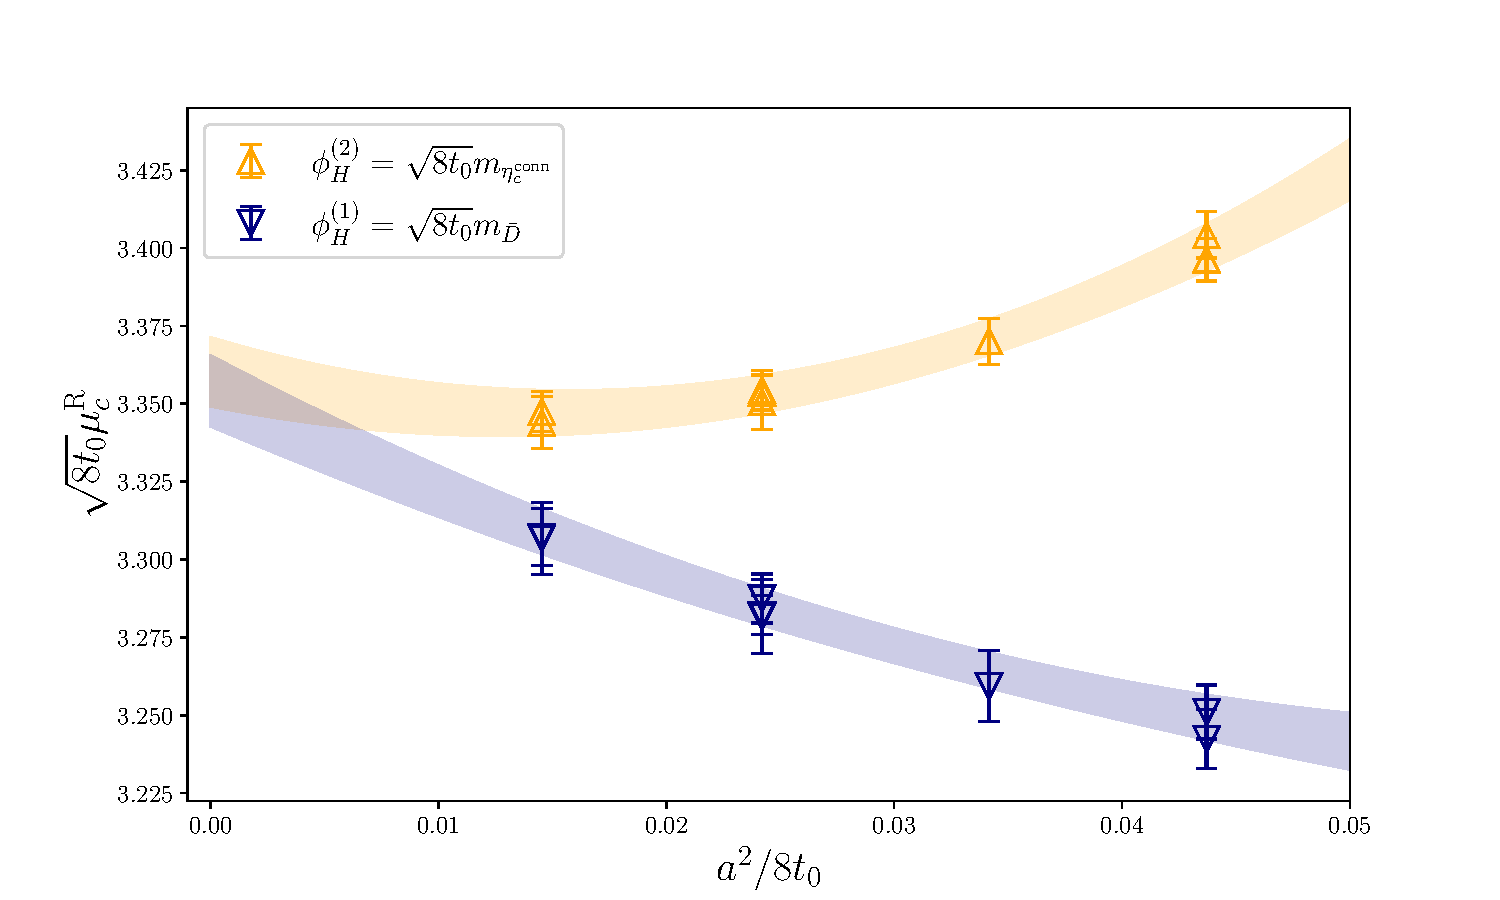
\includegraphics[scale=0.45]{./cap6/figs/mc/mc_cl_all_cat.pdf}
	\caption{Comparison of the continuum limit approach for the two  charm matching 
	prescriptions. Shown are two of the fits with the highest weights from the TIC, projected onto the lattice 
	spacing dimension. In yellow we show results for the $\eta_h^{\mathrm{conn}}$ matching condition, while  the blue 
	points illustrate  the flavor-averaged matching. Each data-point in this plot is projected to the 
	physical pion mass and the physical charm quark mass, in order to properly visualize the lattice 
	spacing dependence. }
	\label{fig:mc_continuum_limit}
\end{figure}

\begin{figure}
	\centering
	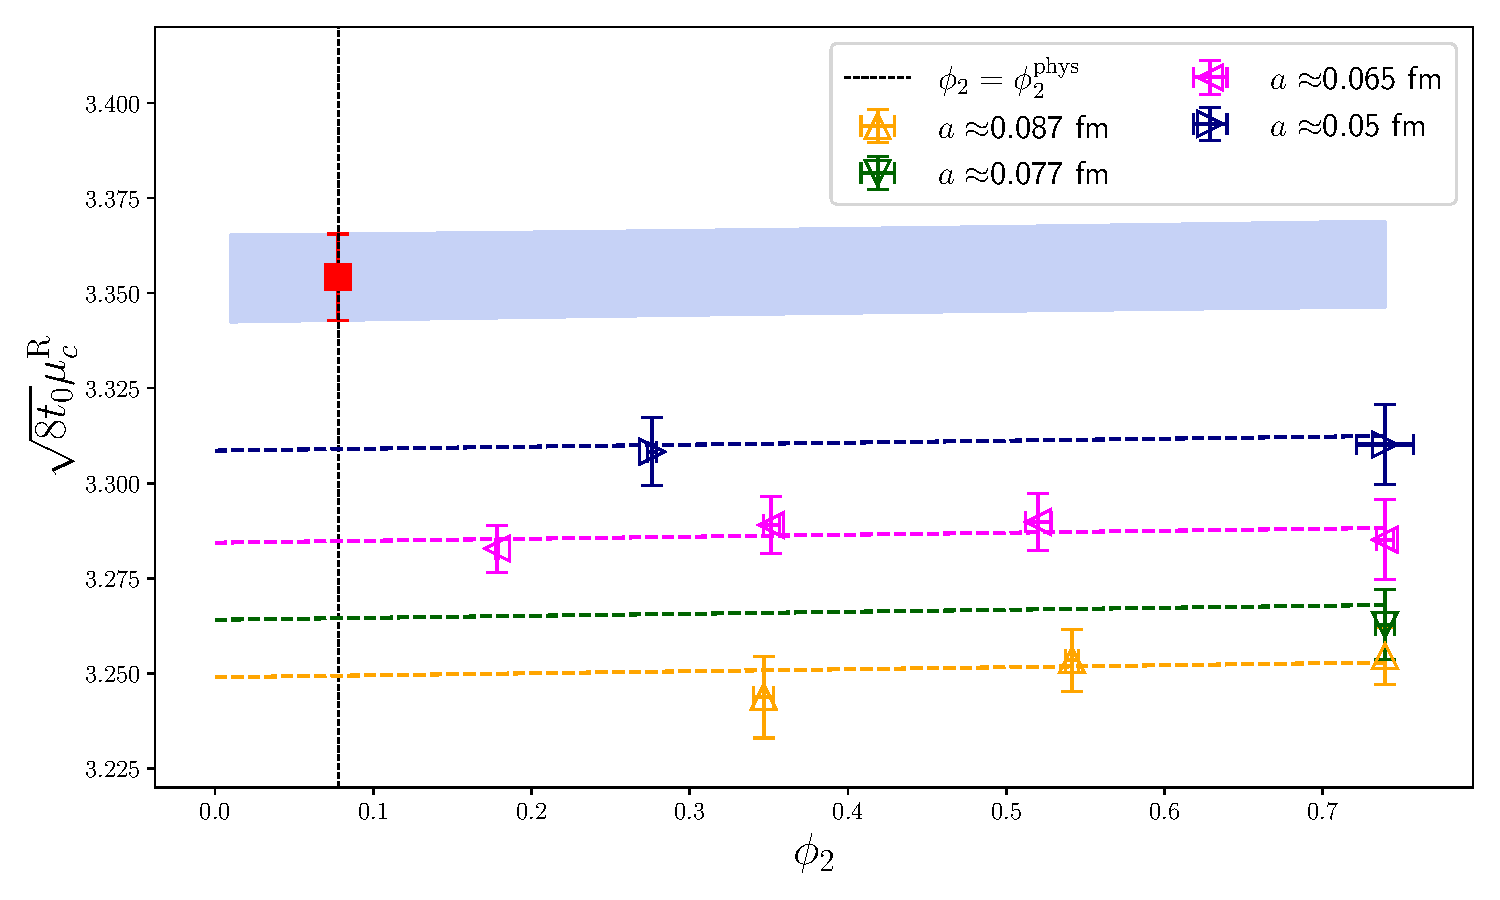
\includegraphics[scale=0.42]{./cap6/figs/mc/fit_phi2_muc_fl_ave.pdf}
	\caption{Pion mass dependence of the charm quark mass for one of the best  fits according to the TIC criteria. Results are shown for the flavor-averaged matching condition. Each point corresponds to the  value for a given ensemble, projected to the physical charm quark mass. The dashed lines represent the chiral trajectories at finite lattice spacing, while the blue shaded band is a projection to the continuum limit. The red point shows our final result extrapolated at the physical point in the continuum. }
	\label{fig:mc_pion_dependence}
\end{figure}

\begin{figure}
 	\centering
 	%\hspace{-15mm}
 	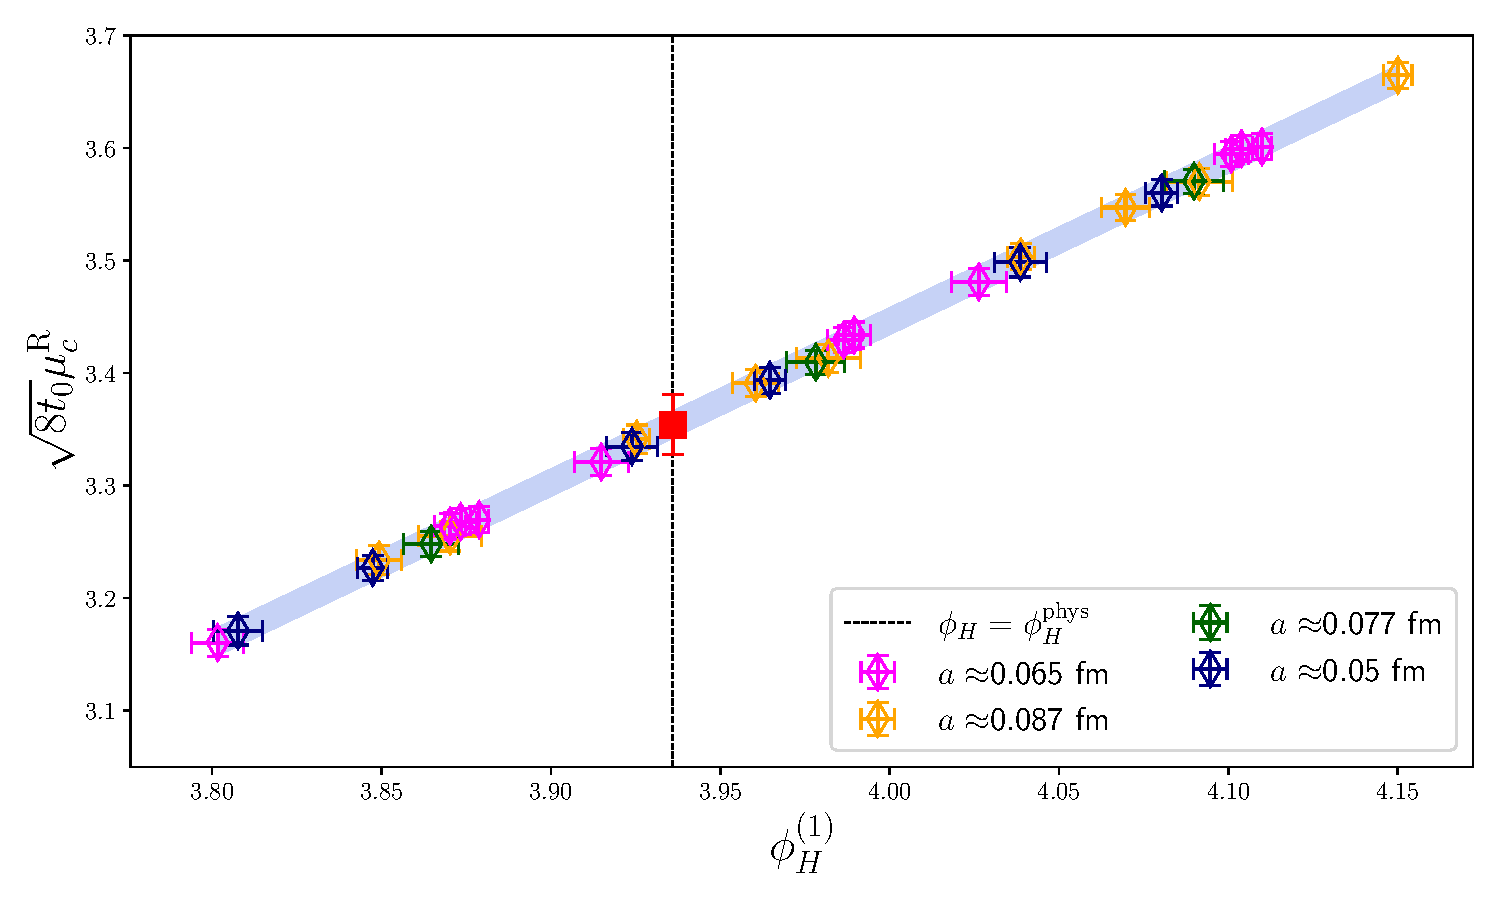
\includegraphics[scale=0.5]{./cap6/figs/mc/fit_phih_interp_muc_fl_ave.pdf}
 	\caption{ Heavy mass dependence of the renormalized charm quark mass $\mu_c^{R}$ in units of $\sqrt{8t_0}$ for one of the fits with larger weights according to the TIC criteria. Results shown for the flavor-averaged matching condition $\phi_{H}^{(1)} = \sqrt{8t_0} m_{\overline{H}}$. Dependencies other than $\phi_H^{(i)}$ in the chiral-continuum extrapolation have been projected to the physical point. The red square symbols indicate the continuum results at the physical value $\phi_H^{\mathrm{ph}}$. We observe a linear dependence of the charm quark mass on $\phi_{H}^{(1)} = \sqrt{8t_0} m_{\overline{H}}$. }
 	\label{fig:mc_mh_dependence}
 \end{figure}


\subsection{Results for the charm quark mass}

The renormalized charm quark mass 
$\mu_c^{\textrm{R}}$ can be obtained once we combine the results collected in Table~\ref{tab:mc_results_all_matching} with our determination of $\sqrt{t_0^{\mathrm{ph}}}$ in eq.~(\ref{ch_ss:eq:t0ph_c}). As discussed at the beginning of this section, the knowledge of the renormalization group running factors allows  to quote
results for the RGI and $\overline{\textrm{MS}}$ values of the charm quark mass.

After combining the results from our 128 fitting models through the model average procedure,
and using the running factor in eq.~(\ref{eq:rgi_running_factor}), we quote for the three-flavor theory
the value for the RGI quark mass
\begin{equation}
  M_c^{\mathrm{RGI}}(N_f=3) &=& 1.485(8)_{\textrm{stat}}(3)_{\textrm{syst}}(14)_{\textrm{RGI}}\ \mathrm{GeV}\,,
	\label{eq:rgi_charm_mass_result}
\end{equation}
where the first error is statistical, including the uncertainty on  $t_0^{\mathrm{ph}}$,  the second accounts for the systematic uncertainty, derived from the model average, and the third is the error contribution from the RGI running factor in eq.~(\ref{eq:rgi_running_factor}). 

Figure~\ref{fig:mc_error_contributions} illustrates the relative contribution of various sources of error to the
uncertainty of our determination of $M_c^{\mathrm{RGI}}$. The dominant source of error comes from the 
renormalization group running of eq.~(\ref{eq:rgi_running_factor}), while the second most relevant 
contribution arises from the statistical error of  the correlation functions computed in each ensemble.  
The  error coming from  the uncertainty on $t_0^{\mathrm{ph}}$ based on our  scale setting  procedure, as well as the 
systematic error from the model average  are subleading contributions. We therefore expect
that the 
inclusion in this charm quark mass analysis of further ensembles or increased statistics will only have a significant impact if combined with improved determinations of the RGI running factor and the scale setting procedure.
%
\begin{figure}
	\centering
	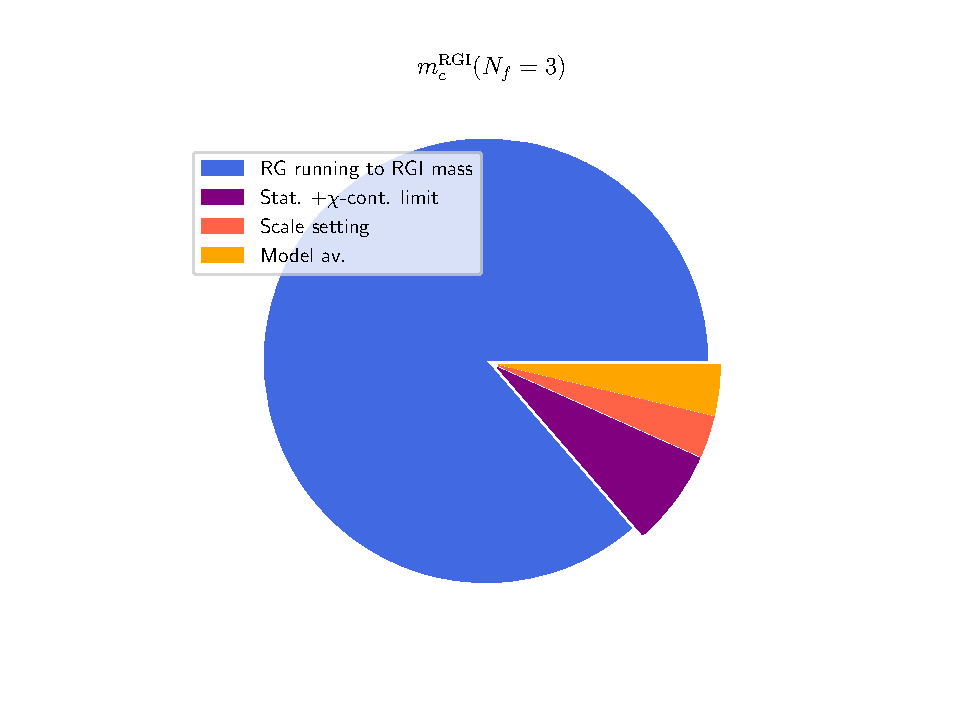
\includegraphics[scale=0.5]{./cap6/figs/mc/mc_error_pie.pdf}
	\caption{Relative contributions to the total variance of our final result for $M_c^{\mathrm{RGI}}$. The dominant piece comes from the error in the non-perturbative determination of the renormalization group running factor to the RGI mass quoted in eq.~(\ref{eq:rgi_running_factor}). The label statistical plus $\chi$-continuum limit stands for the error arising from the statistical accuracy of our data and the chiral-continuum extrapolation, while the scale setting piece comes from the physical value of the gradient flow scale $t_0^{\mathrm{ph}}$. Finally, the model average piece illustrates the systematic error arising from the set of models considered in this work.
          }
	\label{fig:mc_error_contributions}
\end{figure}
%

In order to quote results in the $\overline{\textrm{MS}}$ scheme, we use five-loop perturbation theory for the quark
mass anomalous dimension~\cite{Baikov:2014qja,Luthe:2016xec,Baikov:2017ujl} and the beta function~\cite{Baikov:2016tgj,Herzog:2017ohr,Luthe:2017ttc}.
The matching between the $N_f=3$ and $N_f=4$ theories uses the four-loop decoupling effects~\cite{Liu:2015fxa}
incorporated into the RunDec package~\cite{Chetyrkin:2000yt,Schmidt:2012az,Herren:2017osy}. renormalization group equations are solved using as input the value 
$\Lambda^{(3)}_{\overline{\mathrm{MS}}} = 341(12)\ \mathrm{MeV}$ from~\cite{Bruno:2017gxd}. The correlation arising from the fact that a common subset of gauge field configuration ensembles were employed in the computation of $\Lambda^{(3)}_{\overline{\mathrm{MS}}}$ and the non-perturbative running factor in eq.~(\ref{eq:rgi_running_factor}) is taken into account. We thus arrive to the following results for the RGI and $\overline{\textrm{MS}}$-scheme charm quark masses in the 4-flavor theory,
\begin{align}
  &M_c^{\mathrm{RGI}}(N_f=4)=1.546(8)(3)(14)(4)_\Lambda(3)_{\rm trunc.} \ \mathrm{GeV},\\
  &\overline{m}_c(\mu=3\ \mathrm{GeV}, N_f=4)=1.006(5)(2)(9)(6)_\Lambda(3)_{\rm trunc.} \ \mathrm{GeV},
\end{align}
where the first and second errors arise from the statistical and systematic errors, respectively, in the value of $M_c^{\mathrm{RGI}}(N_f=3)$ in eq.~(\ref{eq:rgi_charm_mass_result}), the third error is due to the non-perturbative running factor in eq.~(\ref{eq:rgi_running_factor}), the fourth error is related to the uncertainty in $\Lambda^{(3)}_{\overline{\mathrm{MS}}}$, and the fifth error is an estimate of the truncation uncertainty from the deviation between the 5-loop and 4-loop results. 

In Figure~\ref{fig:mc_comparison} we compare our determinations of the charm quark mass in the $\overline{\textrm{MS}}$ scheme with the results from other lattice QCD calculations also based on $N_f=2+1$ dynamical simulations and with the corresponding FLAG average~\cite{FlavourLatticeAveragingGroupFLAG:2021npn}. We observe in particular a good agreement with the results from \cite{Heitger:2021apz} which are also based on CLS ensembles but employ Wilson fermions in the valence sector.

\begin{figure}
	\centering
	\hspace{-0mm}
	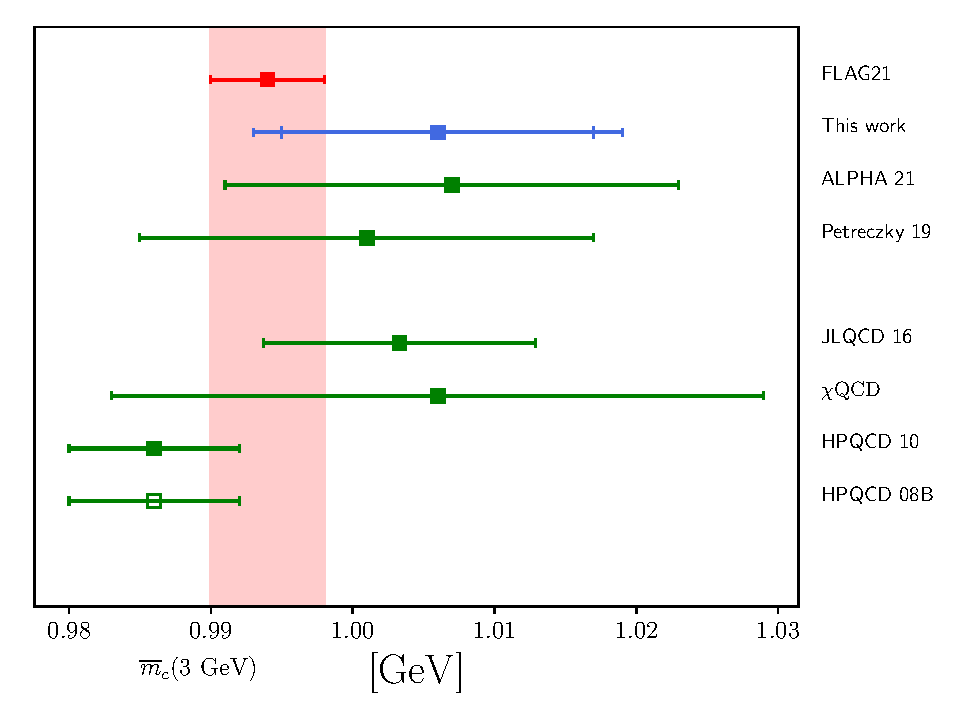
\includegraphics[scale=0.6]{./cap6/figs/mc/mc_comparison_3gev.pdf}
	\caption{Comparison of our charm quark mass determinations in the $\overline{\textrm{MS}}$ scheme with the FLAG average~\cite{FlavourLatticeAveragingGroupFLAG:2021npn} and the results from other lattice QCD calculations based on $N_f=2+1$ dynamical simulations. In our results, shown in blue, we indicate both the total uncertainty and the error when excluding the uncertainty arising from $\Lambda^{(3)}_{\overline{\mathrm{MS}}}$. \textit{Top}: comparison for the  $\overline{m}_c(\mu=3\ \mathrm{GeV}, N_f=4)$. \textit{Bottom}: comparison for $\overline{m}_c(\mu=\overline{m}_c, N_f=4)$.  Starting from the bottom, results are taken from: PDG \cite{ParticleDataGroup:2022pth}, HPQCD 08B \cite{HPQCD:2008kxl}, HPQCD 10 \cite{McNeile:2010ji}, $\chi$QCD \cite{Yang:2014sea}, JLQCD 16 \cite{Nakayama:2016atf}, Maezawa 16 \cite{Maezawa:2016vgv}, Petreczky 19 \cite{Petreczky:2019ozv}, ALPHA 21 \cite{Heitger:2021apz}.
       }
	\label{fig:mc_comparison}
\end{figure}

%%%%%%%%%%%%%%%%%%%%%%%%%%%%%%%%%%%%%%%%%%%%%%%%%%%%%%%%%%%
%%%%%%%%%%%%%%%%%%%%%%%%%%%%%%%%%%%%%%%%%%%%%%%%%%%%%%%%%%%
%%%%%%%%%%%%%%%%%%%%%%%%%%%%%%%%%%%%%%%%%%%%%%%%%%%%%%%%%%%
%%%%%%%%%%%%%%%%%%%%%%%%%%%%%%%%%%%%%%%%%%%%%%%%%%%%%%%%%%%


\section{Determination of decay constants of charmed mesons}
\label{sec:fDs}

For the determination of the decay constants of the charmed mesons $D_{(s)}$ we employ a similar methodology to the one for the renormalized charm quark mass. We match the charm quark mass to its physical value following the same prescription as in Sec.~\ref{sec:matching_charm}, and we explore different ways of performing the chiral-continuum limit extrapolations in order to obtain $f_{D_{(s)}}$ at the physical point. For a detailed discussion we refer to our work~\citep{charm}, here we will only show our main results emphasizing the impact on these of our determination of the scale $t_0$ in Chapter \ref{ch_ss}.

\subsection{Computation of decay constants}

The quantity we employ to extract $f_{D_{(s)}}$ in the continuum and at physical quark masses is
\begin{equation}
  \Phi_{D_{(s)}} = (8t_0)^{3/4}f_{D_{(s)}} \sqrt{m_{D_{(s)}}},
  \label{eq:defphiD}
\end{equation}
for which a Heavy Quark Effective Theory (HQET) scaling law in powers of the inverse
heavy quark mass exists.
The general continuum heavy and light quark mass dependence can be expressed as the product of the individual contributions to arrive at the generic expression 
\begin{equation}
	\Phi_{D_{(s)}} = \Phi_{\chi} \left[
	1 + \delta\Phi_{\chi\mathrm{PT}}^{D_{(s)}}
	\right]
	\left[
	1 + \delta\Phi_a^{D_{(s)}}
	\right]\,.
	\label{eq:fds_different_pieces}
\end{equation}
Here $\Phi_\chi$ governs the heavy-quark mass dependence while  $\delta\Phi_{\chi\mathrm{PT}}^{D_{(s)}}$ controls the light quark behavior as approaching the physical point. Finally the lattice spacing dependence describing cut-off effects is regulated by $\delta\Phi_a^{D_{(s)}}$. 

For an analysis of each of the terms appearing in eq.~(\ref{eq:fds_different_pieces}) we refer to our work~\citep{charm}. In particular, we refer to eq. (5.13) in the previously cited work.

Here we only comment that for $\Phi_{\chi}$ we use expressions motivated by HQET, while the light-quark dependence in $\delta\Phi_{\chi\mathrm{PT}}^{D_{(s)}}$ admits an expression in Heavy Meson $\chi$PT (HM$\chi$PT). For cutoff effects, we consider $\mathcal{O}(a^2)$, $\mathcal{O}(a^2\phi_2)$ and $\mathcal{O}(a^2\phi_H)$ terms.

Similarly to the case of the charm quark mass, we consider several specific forms of the fit ansatz,
by setting some combination of fit parameters to zero. We furthermore again match the charm scale using
the two different procedures described in Sec.~\ref{sec:matching_charm}. The result is a total
of 57 different models  for each matching condition,
and we use our TIC criterion to extract a systematic uncertainty associated to the variation
within the full set of fits.

In Table~\ref{tab:dec_res_all_matching} we show our determinations of $\Phi_D$
and $\Phi_{D_s}$ for each of the two procedures to match the charm scale, as well
as the result from their combination. Using this combination we arrive at the following results for the $D_{(s)}$ meson decay constants,
\begin{align}
	f_D &= 211.3(1.9)_{\textrm{stat}}(0.6)_{\textrm{syst} \ \mathrm{MeV},
	\\
	f_{D_s} &= 247.0(1.9)_{\textrm{stat}(0.7)_{\textrm{syst} \ \mathrm{MeV},
\end{align}
where the first error is statistical and the second the systematic uncertainty from the model average. The different contributions to the variance of $D_{(s)}$ meson decay constants are 
shown in Figure~\ref{fig:fds_error_sources}. Finally, in  Figure~\ref{fig:fds_comparison} we show a comparison between our results and other $N_f=2+1$ lattice QCD determinations.
%

\begin{longtable}{c | c c c}
\toprule
&  $\phi_{H}^{(1)}$ & $\phi_{H}^{(2)} $  &  \text{combined} \\
\midrule
$\Phi_D$ &  0.8624(78)(7) & 0.8583(75)(8) &   0.8606(76)(21) \\
$\Phi_{D_s}$ & 1.0352(61)(9) & 1.0295(60)(11) &  1.0328(60)(30) \\
\bottomrule
\caption{Model average results for the observables $\Phi_D$ and $\Phi_{D_s}$ --- defined in eq.~(\ref{eq:defphiD}) ---  which are related to the $f_D$ and $f_{D_s}$ decay constants, respectively, for
		the two different matching quantities $\phi_H^{(i)}$. The last column reports the result of the combination of these two matching conditions. The first error is statistical while the second is the estimate of systematic uncertainty arising from the model averaging procedure. }
		\label{tab:dec_res_all_matching}
\end{longtable}

\begin{figure}
\begin{center}
\begin{minipage}{.40\linewidth}
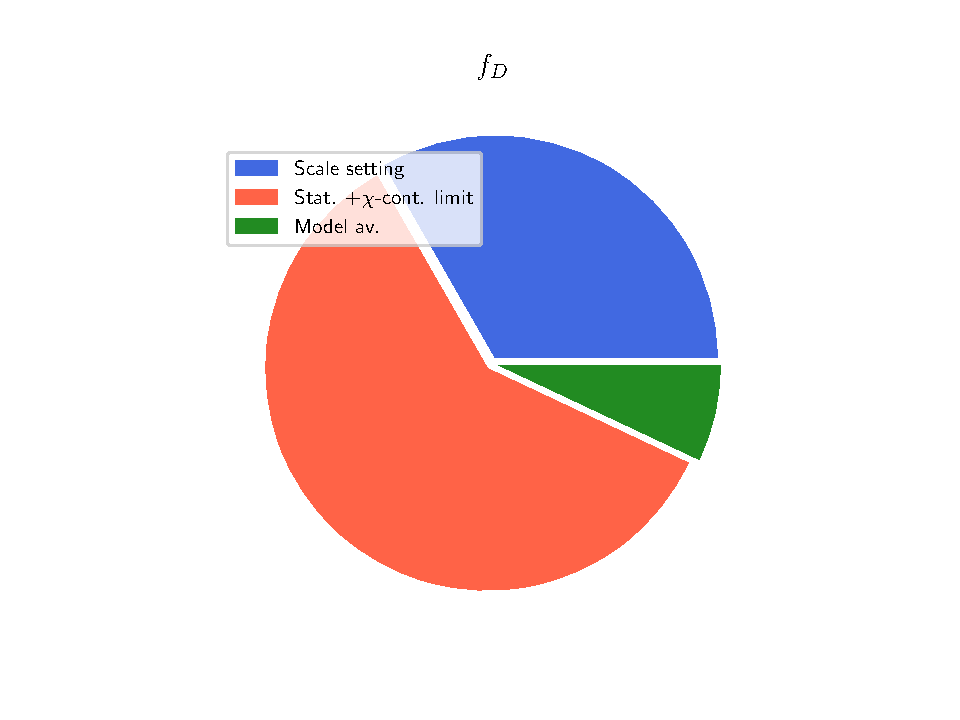
\includegraphics[width=\linewidth]{././cap6/figs/fds/error_pie_fd.pdf}
\end{minipage}
\hspace{10mm}
\begin{minipage}{.39\linewidth}
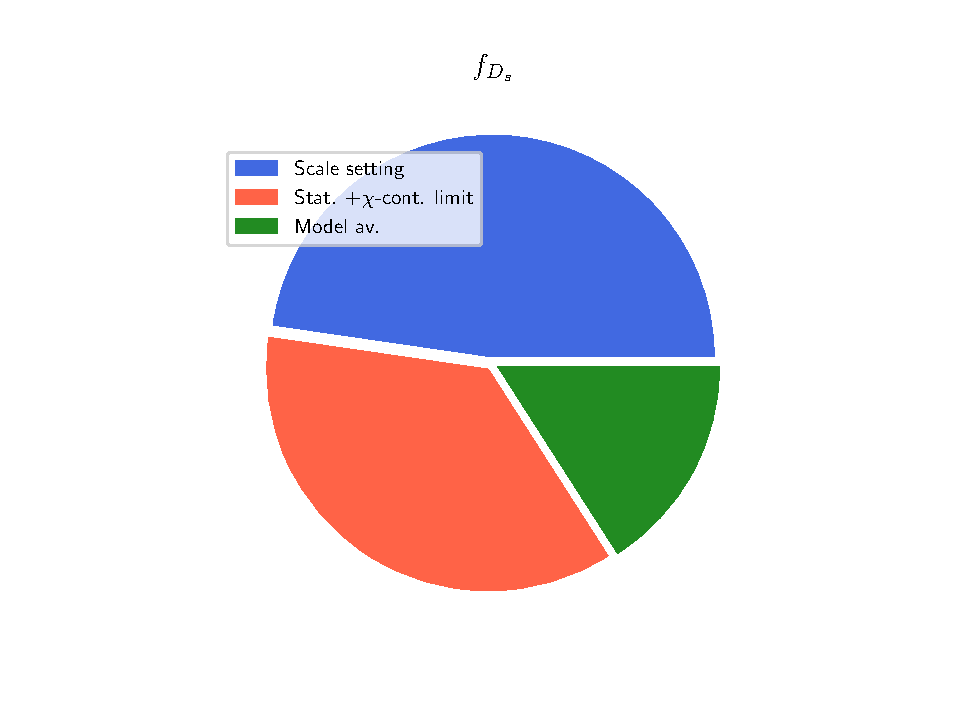
\includegraphics[width=\linewidth]{././cap6/figs/fds/error_pie_fds.pdf}
\end{minipage}
\end{center}
\vspace{-5mm}
	\caption{Relative contributions to the total error of our determinations of $f_D$ (\textit{left}) and $f_{D_s}$ (\textit{right}). The label statistical plus $\chi$-continuum limit represents the error arising from the statistical accuracy of our data and the chiral-continuum extrapolations. The scale setting label denotes the error coming from the physical value $t_0^{\mathrm{ph}}$ as determined in Chapter \ref{ch_ss}, while the model average represents the systematic error arising from the model variation according to the TIC procedure.	}
	\label{fig:fds_error_sources}
\end{figure}


\begin{figure}
	\centering
	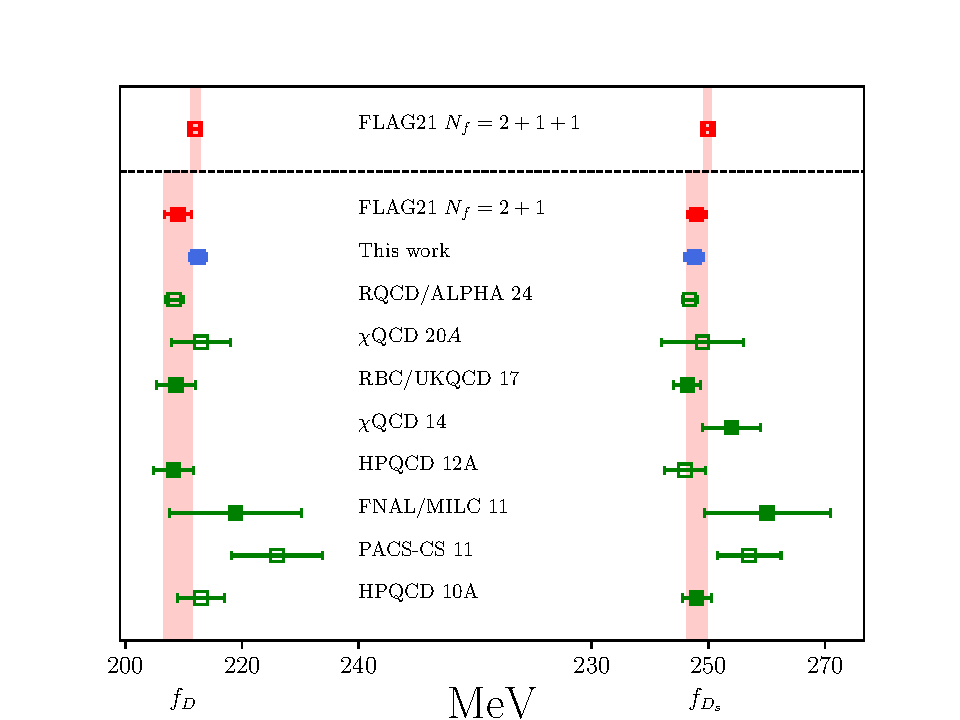
\includegraphics[scale=0.70]{./cap6/figs/fds/fds_comparison.pdf}
	\caption{Comparison of our results for $f_D$ and $f_{D_s}$  with those from lattice QCD collaborations based on simulations with $N_f=2+1$ dynamical flavors as well as with FLAG21 averages~\cite{FlavourLatticeAveragingGroupFLAG:2021npn}.
          Only data points with filled symbols contribute to  the FLAG averages. Starting from the bottom, results are taken from: HPQCD 10 \cite{Davies:2010ip}, PACS-CS 11 \cite{PACS-CS:2011ngu}, FNAL/MILC 11 \cite{FermilabLattice:2011njy}, HPQCD 12A \cite{Na:2012iu}, $\chi$QCD 14 \cite{Yang:2014sea}, RBC/UKQCD 17 \cite{Boyle:2017jwu},  $\chi$QCD 20A \cite{Chen:2020qma}.
          }
	\label{fig:fds_comparison}
\end{figure}


\subsection{Direct determination of $f_{D_s}/f_D$}

In addition to the determination of $f_D$ and $f_{D_s}$, we investigate the direct determination
of the ratio $f_{D_s}/f_D$ from a dedicated fit. This allows for a consistency check, since
the ratio is dimensionless and thus does not require normalization with a reference scale
such as $\sqrt{8t_0}$. One particular consequence is thus that this approach is only
indirectly subject to the uncertainty of the lattice scale setting. Another advantage
is that the ratio is exactly~1 by construction when $m_s=m_l$, i.e., the symmetric
point of our $\phi_4={\rm const.}$ trajectory, which is part of our line of constant
physics. We can thus perform a fit that is highly constrained in the unphysical masses
region, although at the price of reducing the total number of ensembles entering in the study of the approach to the physical point.

A first set of fit ansaetze is derived from HM$\chi$PT expressions as in the case
for $\Phi_{D_{(s)}}$. The generic form is
\begin{equation}
	\frac{\Phi_{D_s}}{\Phi_D} = \left[
	1 + \left(
	\delta\Phi_{\chi\mathrm{PT}}^{D_s} - \delta\Phi_{\chi\mathrm{PT}}^{D}
	\right)
	\right]
	\left[
	1 + \left(
	\delta\Phi_{a}^{D_s} - \delta\Phi_{a}^{D_s}
	\right)
	\right].
	\label{eq:ratio_fds_expansion}
\end{equation}
Here $\delta\Phi_{\chi\mathrm{PT}}^{D_{(s)}}$ labels the light quark mass dependence of the ratio, while $\delta\Phi_a^{D_{(s)}}$ controls the continuum approach. For more details we refer to eq. (5.18) in~\citep{charm}.
In the expression for $\frac{\Phi_{D_s}}{\Phi_D}$ we consider all the possible combinations of non-vanishing fit parameters,
and perform our TIC-weighted model average among the different functional forms tested to
quote a systematic uncertainty.  

We further explore the systematic uncertainties by considering  also functional forms based on a Taylor expansion of $\Phi_{D_{(s)}}$. The generic
expression then reads
\begin{align}
	\Phi_{D_{(s)}}= \left( \Phi_{D_{(s)}}\right)_{\chi} \left[ 1 + \delta \Phi_{{h,\mathrm{Taylor}}} \right] \left[ 1 + \delta \Phi_{{m,\mathrm{Taylor}}}^{D_{(s)}} \right] \left[ 1 + \delta \Phi_a^{D_{(s)}}  \right]
	\,,
	\label{eq:phiqcontT}
\end{align}
where $ \left( \Phi_{D_{(s)}}\right)_{\chi}$ is the value in
the chiral limit and at the physical value of the heavy-quark mass. More concretely, we refer to eq. (5.21) in~\citep{charm}.


Then, in order to arrive at a final determination of $f_{D_s}/f_D$ we perform a model average among all the HM$\chi$PT and Taylor functional forms, considering all the possible combinations of non-vanishing fit parameters, for the two different matching conditions simultaneously. In Table~\ref{tab:ratio_res_all_matching} we report our results for the
ratio of decay constants from the model average separately for each charm matching
condition, as well as their combination. Also for the ratio we observe good agreement for the two different $\phi_H^{(i)}$ tested in this work. 
Finally, for the  result combining the two matching conditions, we quote 
\begin{equation}
	\frac{f_{D_s}}{f_D} = 1.177(15)_{\textrm{stat}(5)_{\textrm{syst},
\end{equation}
where  the first error is  statistical and the second is the systematic uncertainty based on  the model average procedure. 


\begin{longtable}{c | c c c}
\toprule
&  $\phi_{H}^{(1)}$ & $\phi_{H}^{(2)} $  &  \text{combined} \\
\midrule
$f_{D_s}/f_D$   &  1.177(15)(6)& 1.178(15)(6) &  1.177(15)(5) \\
\bottomrule
\caption{Results of the model average for $f_{D_s}/f_D$ for the two charm-quark matching conditions. The last column reports the combined result. The first error is statistical while the second is the systematic uncertainty arising from the model variation procedure. }
		\label{tab:ratio_res_all_matching}
\end{longtable}

  In Figure \ref{fig:fds_ratio_error}  we show the major error sources contributing to our final determination of the ratio, where we notice that the major contribution is given by the statistical and chiral-continuum error. Finally, in Figure \ref{fig:fds_over_fd_comparison} we show a comparison between our result for $f_{D_s}/f_D$, the FLAG21 average and results from other collaborations.


\begin{figure}
\begin{center}
\begin{minipage}{.4\linewidth}
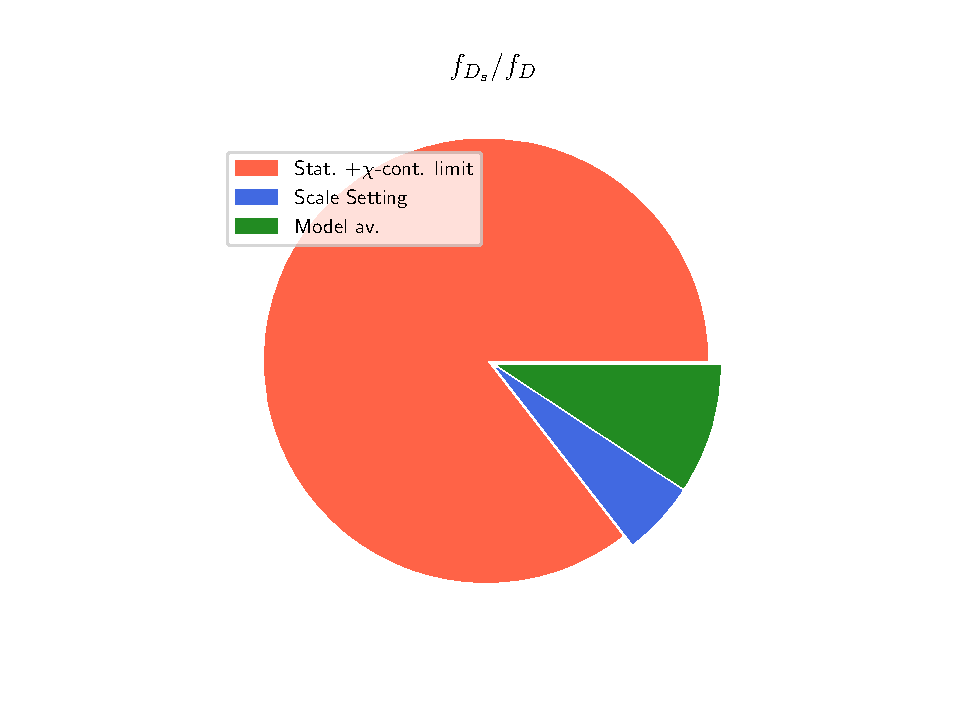
\includegraphics[width=\linewidth]{././cap6/figs/fds/error_pie_ratio_fds.pdf}
\end{minipage}
\hspace{15mm}
\begin{minipage}{.37\linewidth}
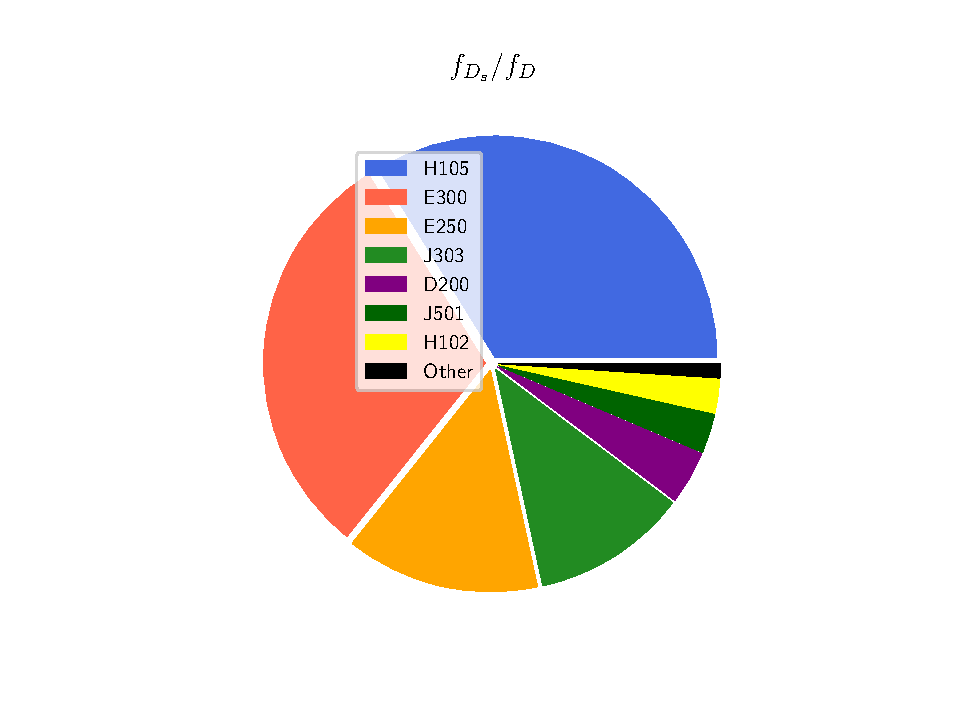
\includegraphics[width=\linewidth]{././cap6/figs/fds/error_pie_ratio_fds_statonly.pdf}
\end{minipage}
\end{center}
\vspace{-5mm}
	\caption{\textit{Left}: Relative contributions to the total error on the determination of the ratio $f_{D_s}/f_D$. The label statistical plus $\chi$-continuum limit represents the error arising from the statistical accuracy of our data and the chiral-continuum extrapolation. The scale setting label denotes the error coming from the physical value $t_0^{\mathrm{ph}}$, while the model average represents the systematic error arising from the model variation according to the TIC procedure. \textit{Right}: Details of the relative contributions to the statistical and chiral-continuum extrapolation error arising from specific gauge field configuration ensembles. 
          }
	    \label{fig:fds_ratio_error}
\end{figure}

\begin{figure}
	\centering
	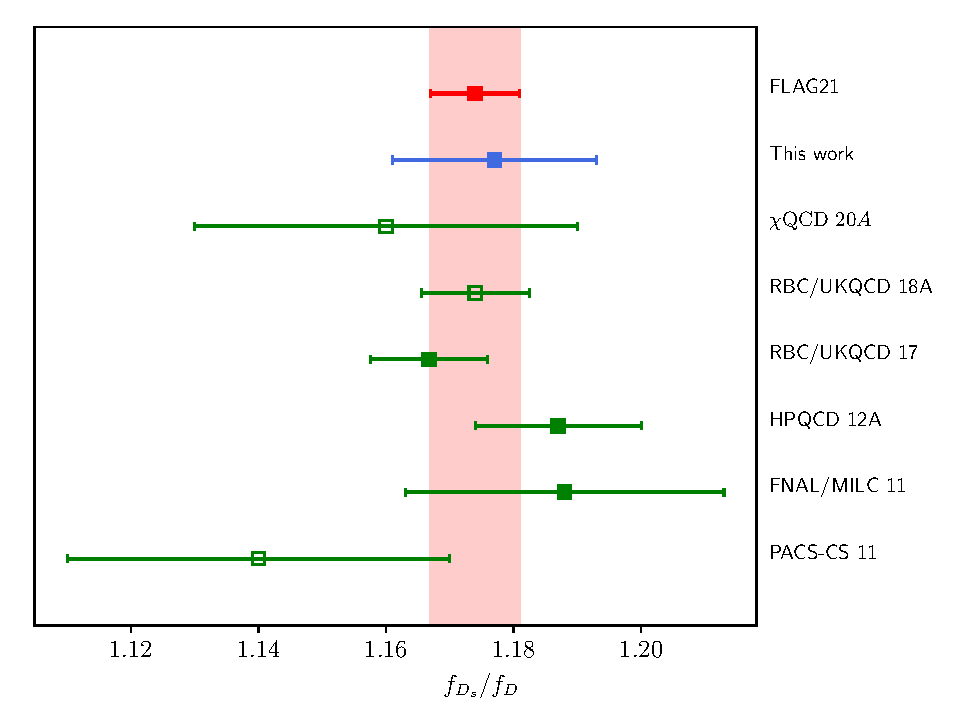
\includegraphics[scale=0.7]{./cap6/figs/fds/ratio_fds_comparison.pdf}
	\caption{Comparison of our determination of $f_{D_s}/f_D$ with those of the other lattice QCD collaborations based on $N_f=2+1$ dynamical simulations as well as with the FLAG average~\cite{FlavourLatticeAveragingGroupFLAG:2021npn}. Only the results with filled symbols contribute to this average. Starting from the bottom, results are taken from:  PACS-CS 11 \cite{PACS-CS:2011ngu}, FNAL/MILC 11  \cite{FermilabLattice:2011njy}, HPQCD 12A \cite{Na:2012iu},  RBC/UKQCD 17 \cite{Boyle:2017jwu}, RBC/UKQCD 18A \cite{Boyle:2018knm},  $\chi$QCD 20A \cite{Chen:2020qma}. }
	\label{fig:fds_over_fd_comparison}
\end{figure}





%%%%%%%%%%%%%%%%%%%%%%%%%%%%%%%%%%%%%%%%%%%%%%%%%%%%%%%%%%%
%%%%%%%%%%%%%%%%%%%%%%%%%%%%%%%%%%%%%%%%%%%%%%%%%%%%%%%%%%%
